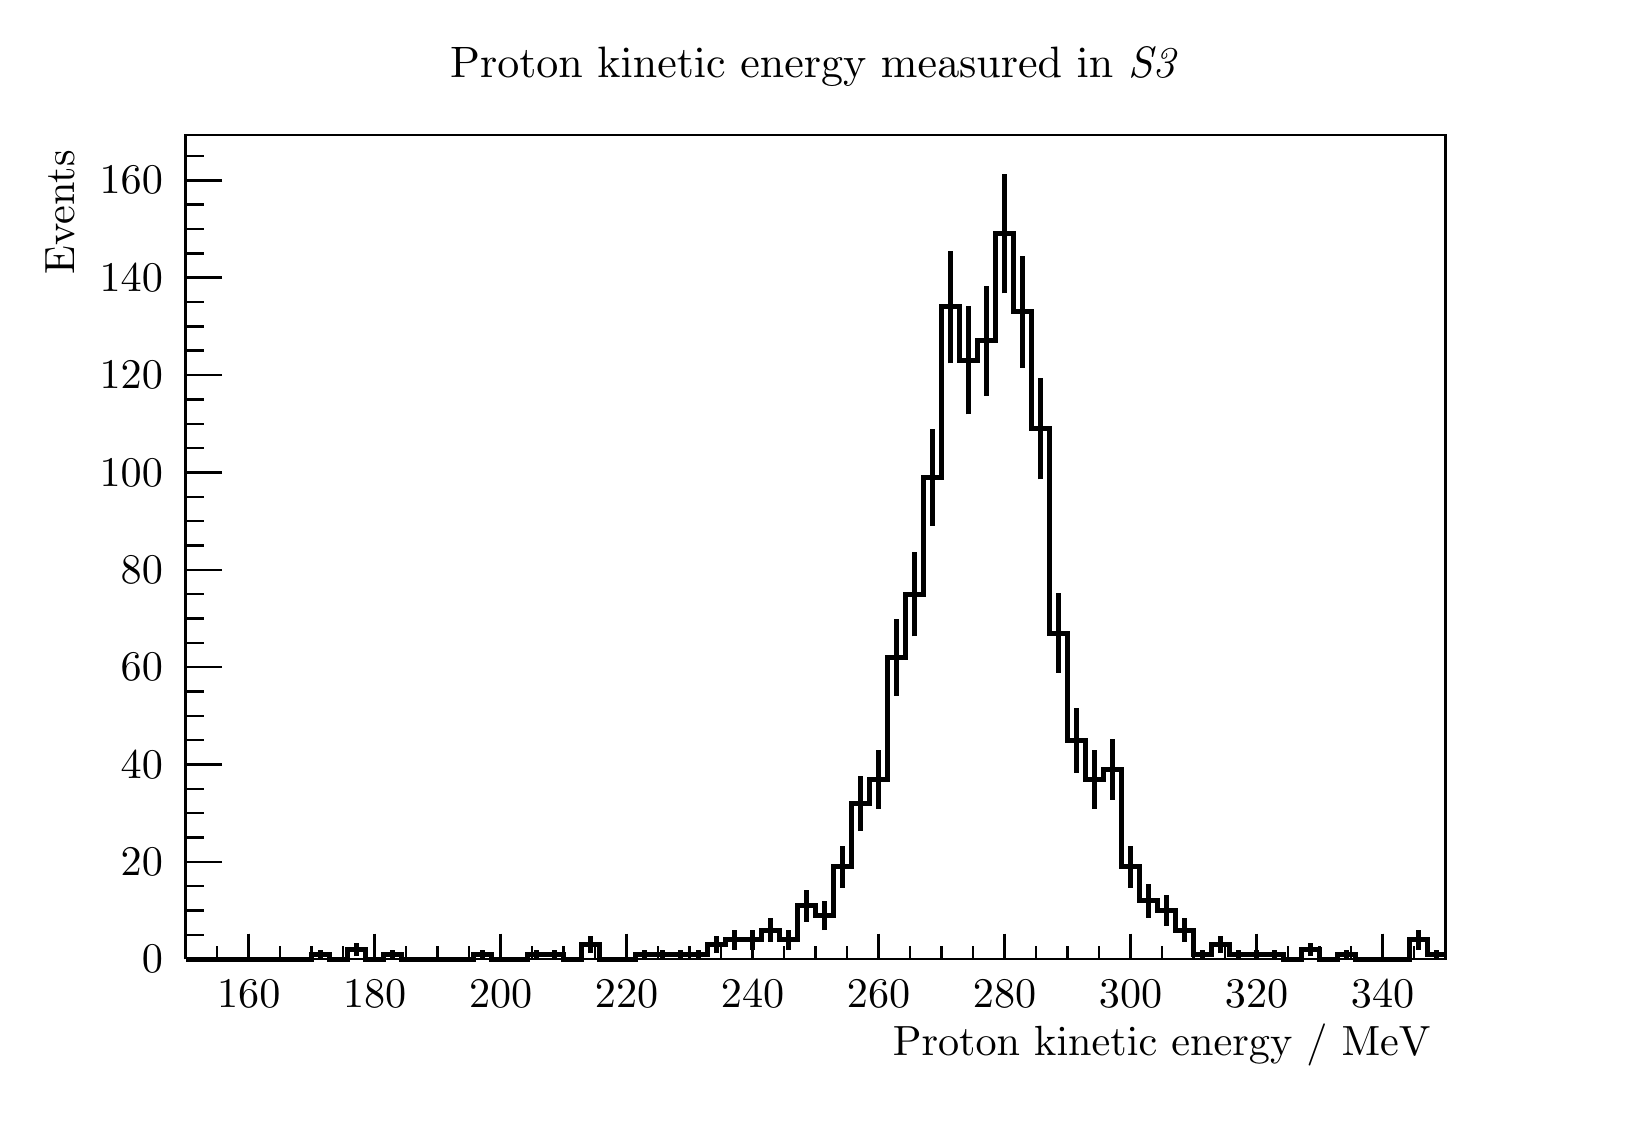
\begin{tikzpicture}
\pgfdeclareplotmark{cross} {
\pgfpathmoveto{\pgfpoint{-0.3\pgfplotmarksize}{\pgfplotmarksize}}
\pgfpathlineto{\pgfpoint{+0.3\pgfplotmarksize}{\pgfplotmarksize}}
\pgfpathlineto{\pgfpoint{+0.3\pgfplotmarksize}{0.3\pgfplotmarksize}}
\pgfpathlineto{\pgfpoint{+1\pgfplotmarksize}{0.3\pgfplotmarksize}}
\pgfpathlineto{\pgfpoint{+1\pgfplotmarksize}{-0.3\pgfplotmarksize}}
\pgfpathlineto{\pgfpoint{+0.3\pgfplotmarksize}{-0.3\pgfplotmarksize}}
\pgfpathlineto{\pgfpoint{+0.3\pgfplotmarksize}{-1.\pgfplotmarksize}}
\pgfpathlineto{\pgfpoint{-0.3\pgfplotmarksize}{-1.\pgfplotmarksize}}
\pgfpathlineto{\pgfpoint{-0.3\pgfplotmarksize}{-0.3\pgfplotmarksize}}
\pgfpathlineto{\pgfpoint{-1.\pgfplotmarksize}{-0.3\pgfplotmarksize}}
\pgfpathlineto{\pgfpoint{-1.\pgfplotmarksize}{0.3\pgfplotmarksize}}
\pgfpathlineto{\pgfpoint{-0.3\pgfplotmarksize}{0.3\pgfplotmarksize}}
\pgfpathclose
\pgfusepathqstroke
}
\pgfdeclareplotmark{cross*} {
\pgfpathmoveto{\pgfpoint{-0.3\pgfplotmarksize}{\pgfplotmarksize}}
\pgfpathlineto{\pgfpoint{+0.3\pgfplotmarksize}{\pgfplotmarksize}}
\pgfpathlineto{\pgfpoint{+0.3\pgfplotmarksize}{0.3\pgfplotmarksize}}
\pgfpathlineto{\pgfpoint{+1\pgfplotmarksize}{0.3\pgfplotmarksize}}
\pgfpathlineto{\pgfpoint{+1\pgfplotmarksize}{-0.3\pgfplotmarksize}}
\pgfpathlineto{\pgfpoint{+0.3\pgfplotmarksize}{-0.3\pgfplotmarksize}}
\pgfpathlineto{\pgfpoint{+0.3\pgfplotmarksize}{-1.\pgfplotmarksize}}
\pgfpathlineto{\pgfpoint{-0.3\pgfplotmarksize}{-1.\pgfplotmarksize}}
\pgfpathlineto{\pgfpoint{-0.3\pgfplotmarksize}{-0.3\pgfplotmarksize}}
\pgfpathlineto{\pgfpoint{-1.\pgfplotmarksize}{-0.3\pgfplotmarksize}}
\pgfpathlineto{\pgfpoint{-1.\pgfplotmarksize}{0.3\pgfplotmarksize}}
\pgfpathlineto{\pgfpoint{-0.3\pgfplotmarksize}{0.3\pgfplotmarksize}}
\pgfpathclose
\pgfusepathqfillstroke
}
\pgfdeclareplotmark{newstar} {
\pgfpathmoveto{\pgfqpoint{0pt}{\pgfplotmarksize}}
\pgfpathlineto{\pgfqpointpolar{44}{0.5\pgfplotmarksize}}
\pgfpathlineto{\pgfqpointpolar{18}{\pgfplotmarksize}}
\pgfpathlineto{\pgfqpointpolar{-20}{0.5\pgfplotmarksize}}
\pgfpathlineto{\pgfqpointpolar{-54}{\pgfplotmarksize}}
\pgfpathlineto{\pgfqpointpolar{-90}{0.5\pgfplotmarksize}}
\pgfpathlineto{\pgfqpointpolar{234}{\pgfplotmarksize}}
\pgfpathlineto{\pgfqpointpolar{198}{0.5\pgfplotmarksize}}
\pgfpathlineto{\pgfqpointpolar{162}{\pgfplotmarksize}}
\pgfpathlineto{\pgfqpointpolar{134}{0.5\pgfplotmarksize}}
\pgfpathclose
\pgfusepathqstroke
}
\pgfdeclareplotmark{newstar*} {
\pgfpathmoveto{\pgfqpoint{0pt}{\pgfplotmarksize}}
\pgfpathlineto{\pgfqpointpolar{44}{0.5\pgfplotmarksize}}
\pgfpathlineto{\pgfqpointpolar{18}{\pgfplotmarksize}}
\pgfpathlineto{\pgfqpointpolar{-20}{0.5\pgfplotmarksize}}
\pgfpathlineto{\pgfqpointpolar{-54}{\pgfplotmarksize}}
\pgfpathlineto{\pgfqpointpolar{-90}{0.5\pgfplotmarksize}}
\pgfpathlineto{\pgfqpointpolar{234}{\pgfplotmarksize}}
\pgfpathlineto{\pgfqpointpolar{198}{0.5\pgfplotmarksize}}
\pgfpathlineto{\pgfqpointpolar{162}{\pgfplotmarksize}}
\pgfpathlineto{\pgfqpointpolar{134}{0.5\pgfplotmarksize}}
\pgfpathclose
\pgfusepathqfillstroke
}
\definecolor{c}{rgb}{1,1,1};
\draw [color=c, fill=c] (0,0) rectangle (20,13.5908);
\draw [color=c, fill=c] (2,1.76681) rectangle (18,12.2318);
\definecolor{c}{rgb}{0,0,0};
\draw [c,line width=0.9] (2,1.76681) -- (2,12.2318) -- (18,12.2318) -- (18,1.76681) -- (2,1.76681);
\definecolor{c}{rgb}{1,1,1};
\draw [color=c, fill=c] (2,1.76681) rectangle (18,12.2318);
\definecolor{c}{rgb}{0,0,0};
\draw [c,line width=0.9] (2,1.76681) -- (2,12.2318) -- (18,12.2318) -- (18,1.76681) -- (2,1.76681);
\draw [c,line width=1.8] (3.71429,1.76681) -- (3.71429,1.82863);
\draw [c,line width=1.8] (3.71429,1.82863) -- (3.71429,1.89046);
\foreach \P in {(3.71429,1.82863)}{\draw[mark options={color=c,fill=c},mark size=2.402402pt,mark=*,mark size=1pt] plot coordinates {\P};}
\draw [c,line width=1.8] (4.17143,1.80303) -- (4.17143,1.89046);
\draw [c,line width=1.8] (4.17143,1.89046) -- (4.17143,1.97789);
\foreach \P in {(4.17143,1.89046)}{\draw[mark options={color=c,fill=c},mark size=2.402402pt,mark=*,mark size=1pt] plot coordinates {\P};}
\draw [c,line width=1.8] (4.62857,1.76681) -- (4.62857,1.82863);
\draw [c,line width=1.8] (4.62857,1.82863) -- (4.62857,1.89046);
\foreach \P in {(4.62857,1.82863)}{\draw[mark options={color=c,fill=c},mark size=2.402402pt,mark=*,mark size=1pt] plot coordinates {\P};}
\draw [c,line width=1.8] (5.77143,1.76681) -- (5.77143,1.82863);
\draw [c,line width=1.8] (5.77143,1.82863) -- (5.77143,1.89046);
\foreach \P in {(5.77143,1.82863)}{\draw[mark options={color=c,fill=c},mark size=2.402402pt,mark=*,mark size=1pt] plot coordinates {\P};}
\draw [c,line width=1.8] (6.45714,1.76681) -- (6.45714,1.82863);
\draw [c,line width=1.8] (6.45714,1.82863) -- (6.45714,1.89046);
\foreach \P in {(6.45714,1.82863)}{\draw[mark options={color=c,fill=c},mark size=2.402402pt,mark=*,mark size=1pt] plot coordinates {\P};}
\draw [c,line width=1.8] (6.68571,1.76681) -- (6.68571,1.82863);
\draw [c,line width=1.8] (6.68571,1.82863) -- (6.68571,1.89046);
\foreach \P in {(6.68571,1.82863)}{\draw[mark options={color=c,fill=c},mark size=2.402402pt,mark=*,mark size=1pt] plot coordinates {\P};}
\draw [c,line width=1.8] (7.14286,1.8452) -- (7.14286,1.95229);
\draw [c,line width=1.8] (7.14286,1.95229) -- (7.14286,2.05937);
\foreach \P in {(7.14286,1.95229)}{\draw[mark options={color=c,fill=c},mark size=2.402402pt,mark=*,mark size=1pt] plot coordinates {\P};}
\draw [c,line width=1.8] (7.82857,1.76681) -- (7.82857,1.82863);
\draw [c,line width=1.8] (7.82857,1.82863) -- (7.82857,1.89046);
\foreach \P in {(7.82857,1.82863)}{\draw[mark options={color=c,fill=c},mark size=2.402402pt,mark=*,mark size=1pt] plot coordinates {\P};}
\draw [c,line width=1.8] (8.05714,1.76681) -- (8.05714,1.82863);
\draw [c,line width=1.8] (8.05714,1.82863) -- (8.05714,1.89046);
\foreach \P in {(8.05714,1.82863)}{\draw[mark options={color=c,fill=c},mark size=2.402402pt,mark=*,mark size=1pt] plot coordinates {\P};}
\draw [c,line width=1.8] (8.28571,1.76681) -- (8.28571,1.82863);
\draw [c,line width=1.8] (8.28571,1.82863) -- (8.28571,1.89046);
\foreach \P in {(8.28571,1.82863)}{\draw[mark options={color=c,fill=c},mark size=2.402402pt,mark=*,mark size=1pt] plot coordinates {\P};}
\draw [c,line width=1.8] (8.51429,1.76681) -- (8.51429,1.82863);
\draw [c,line width=1.8] (8.51429,1.82863) -- (8.51429,1.89046);
\foreach \P in {(8.51429,1.82863)}{\draw[mark options={color=c,fill=c},mark size=2.402402pt,mark=*,mark size=1pt] plot coordinates {\P};}
\draw [c,line width=1.8] (8.74286,1.8452) -- (8.74286,1.95229);
\draw [c,line width=1.8] (8.74286,1.95229) -- (8.74286,2.05937);
\foreach \P in {(8.74286,1.95229)}{\draw[mark options={color=c,fill=c},mark size=2.402402pt,mark=*,mark size=1pt] plot coordinates {\P};}
\draw [c,line width=1.8] (8.97143,1.89046) -- (8.97143,2.01411);
\draw [c,line width=1.8] (8.97143,2.01411) -- (8.97143,2.13776);
\foreach \P in {(8.97143,2.01411)}{\draw[mark options={color=c,fill=c},mark size=2.402402pt,mark=*,mark size=1pt] plot coordinates {\P};}
\draw [c,line width=1.8] (9.2,1.89046) -- (9.2,2.01411);
\draw [c,line width=1.8] (9.2,2.01411) -- (9.2,2.13776);
\foreach \P in {(9.2,2.01411)}{\draw[mark options={color=c,fill=c},mark size=2.402402pt,mark=*,mark size=1pt] plot coordinates {\P};}
\draw [c,line width=1.8] (9.42857,1.98632) -- (9.42857,2.13776);
\draw [c,line width=1.8] (9.42857,2.13776) -- (9.42857,2.2892);
\foreach \P in {(9.42857,2.13776)}{\draw[mark options={color=c,fill=c},mark size=2.402402pt,mark=*,mark size=1pt] plot coordinates {\P};}
\draw [c,line width=1.8] (9.65714,1.89046) -- (9.65714,2.01411);
\draw [c,line width=1.8] (9.65714,2.01411) -- (9.65714,2.13776);
\foreach \P in {(9.65714,2.01411)}{\draw[mark options={color=c,fill=c},mark size=2.402402pt,mark=*,mark size=1pt] plot coordinates {\P};}
\draw [c,line width=1.8] (9.88571,2.24184) -- (9.88571,2.44689);
\draw [c,line width=1.8] (9.88571,2.44689) -- (9.88571,2.65194);
\foreach \P in {(9.88571,2.44689)}{\draw[mark options={color=c,fill=c},mark size=2.402402pt,mark=*,mark size=1pt] plot coordinates {\P};}
\draw [c,line width=1.8] (10.1143,2.13776) -- (10.1143,2.32324);
\draw [c,line width=1.8] (10.1143,2.32324) -- (10.1143,2.50871);
\foreach \P in {(10.1143,2.32324)}{\draw[mark options={color=c,fill=c},mark size=2.402402pt,mark=*,mark size=1pt] plot coordinates {\P};}
\draw [c,line width=1.8] (10.3429,2.672) -- (10.3429,2.94149);
\draw [c,line width=1.8] (10.3429,2.94149) -- (10.3429,3.21098);
\foreach \P in {(10.3429,2.94149)}{\draw[mark options={color=c,fill=c},mark size=2.402402pt,mark=*,mark size=1pt] plot coordinates {\P};}
\draw [c,line width=1.8] (10.5714,3.39548) -- (10.5714,3.74521);
\draw [c,line width=1.8] (10.5714,3.74521) -- (10.5714,4.09495);
\foreach \P in {(10.5714,3.74521)}{\draw[mark options={color=c,fill=c},mark size=2.402402pt,mark=*,mark size=1pt] plot coordinates {\P};}
\draw [c,line width=1.8] (10.8,3.67827) -- (10.8,4.05434);
\draw [c,line width=1.8] (10.8,4.05434) -- (10.8,4.43041);
\foreach \P in {(10.8,4.05434)}{\draw[mark options={color=c,fill=c},mark size=2.402402pt,mark=*,mark size=1pt] plot coordinates {\P};}
\draw [c,line width=1.8] (11.0286,5.11316) -- (11.0286,5.59997);
\draw [c,line width=1.8] (11.0286,5.59997) -- (11.0286,6.08678);
\foreach \P in {(11.0286,5.59997)}{\draw[mark options={color=c,fill=c},mark size=2.402402pt,mark=*,mark size=1pt] plot coordinates {\P};}
\draw [c,line width=1.8] (11.2571,5.86827) -- (11.2571,6.4037);
\draw [c,line width=1.8] (11.2571,6.4037) -- (11.2571,6.93912);
\foreach \P in {(11.2571,6.4037)}{\draw[mark options={color=c,fill=c},mark size=2.402402pt,mark=*,mark size=1pt] plot coordinates {\P};}
\draw [c,line width=1.8] (11.4857,7.27235) -- (11.4857,7.8875);
\draw [c,line width=1.8] (11.4857,7.8875) -- (11.4857,8.50265);
\foreach \P in {(11.4857,7.8875)}{\draw[mark options={color=c,fill=c},mark size=2.402402pt,mark=*,mark size=1pt] plot coordinates {\P};}
\draw [c,line width=1.8] (11.7143,9.3357) -- (11.7143,10.0514);
\draw [c,line width=1.8] (11.7143,10.0514) -- (11.7143,10.7671);
\foreach \P in {(11.7143,10.0514)}{\draw[mark options={color=c,fill=c},mark size=2.402402pt,mark=*,mark size=1pt] plot coordinates {\P};}
\draw [c,line width=1.8] (11.9429,8.68563) -- (11.9429,9.3713);
\draw [c,line width=1.8] (11.9429,9.3713) -- (11.9429,10.057);
\foreach \P in {(11.9429,9.3713)}{\draw[mark options={color=c,fill=c},mark size=2.402402pt,mark=*,mark size=1pt] plot coordinates {\P};}
\draw [c,line width=1.8] (12.1714,8.92187) -- (12.1714,9.6186);
\draw [c,line width=1.8] (12.1714,9.6186) -- (12.1714,10.3153);
\foreach \P in {(12.1714,9.6186)}{\draw[mark options={color=c,fill=c},mark size=2.402402pt,mark=*,mark size=1pt] plot coordinates {\P};}
\draw [c,line width=1.8] (12.4,10.2241) -- (12.4,10.9788);
\draw [c,line width=1.8] (12.4,10.9788) -- (12.4,11.7334);
\foreach \P in {(12.4,10.9788)}{\draw[mark options={color=c,fill=c},mark size=2.402402pt,mark=*,mark size=1pt] plot coordinates {\P};}
\draw [c,line width=1.8] (12.6286,9.27655) -- (12.6286,9.98955);
\draw [c,line width=1.8] (12.6286,9.98955) -- (12.6286,10.7026);
\foreach \P in {(12.6286,9.98955)}{\draw[mark options={color=c,fill=c},mark size=2.402402pt,mark=*,mark size=1pt] plot coordinates {\P};}
\draw [c,line width=1.8] (12.8571,7.86028) -- (12.8571,8.50575);
\draw [c,line width=1.8] (12.8571,8.50575) -- (12.8571,9.15122);
\foreach \P in {(12.8571,8.50575)}{\draw[mark options={color=c,fill=c},mark size=2.402402pt,mark=*,mark size=1pt] plot coordinates {\P};}
\draw [c,line width=1.8] (13.0857,5.40303) -- (13.0857,5.90909);
\draw [c,line width=1.8] (13.0857,5.90909) -- (13.0857,6.41516);
\foreach \P in {(13.0857,5.90909)}{\draw[mark options={color=c,fill=c},mark size=2.402402pt,mark=*,mark size=1pt] plot coordinates {\P};}
\draw [c,line width=1.8] (13.3143,4.13421) -- (13.3143,4.54894);
\draw [c,line width=1.8] (13.3143,4.54894) -- (13.3143,4.96368);
\foreach \P in {(13.3143,4.54894)}{\draw[mark options={color=c,fill=c},mark size=2.402402pt,mark=*,mark size=1pt] plot coordinates {\P};}
\draw [c,line width=1.8] (13.5429,3.67827) -- (13.5429,4.05434);
\draw [c,line width=1.8] (13.5429,4.05434) -- (13.5429,4.43041);
\foreach \P in {(13.5429,4.05434)}{\draw[mark options={color=c,fill=c},mark size=2.402402pt,mark=*,mark size=1pt] plot coordinates {\P};}
\draw [c,line width=1.8] (13.7714,3.79189) -- (13.7714,4.17799);
\draw [c,line width=1.8] (13.7714,4.17799) -- (13.7714,4.56409);
\foreach \P in {(13.7714,4.17799)}{\draw[mark options={color=c,fill=c},mark size=2.402402pt,mark=*,mark size=1pt] plot coordinates {\P};}
\draw [c,line width=1.8] (14,2.672) -- (14,2.94149);
\draw [c,line width=1.8] (14,2.94149) -- (14,3.21098);
\foreach \P in {(14,2.94149)}{\draw[mark options={color=c,fill=c},mark size=2.402402pt,mark=*,mark size=1pt] plot coordinates {\P};}
\draw [c,line width=1.8] (14.2286,2.29454) -- (14.2286,2.50871);
\draw [c,line width=1.8] (14.2286,2.50871) -- (14.2286,2.72288);
\foreach \P in {(14.2286,2.50871)}{\draw[mark options={color=c,fill=c},mark size=2.402402pt,mark=*,mark size=1pt] plot coordinates {\P};}
\draw [c,line width=1.8] (14.4571,2.18955) -- (14.4571,2.38506);
\draw [c,line width=1.8] (14.4571,2.38506) -- (14.4571,2.58057);
\foreach \P in {(14.4571,2.38506)}{\draw[mark options={color=c,fill=c},mark size=2.402402pt,mark=*,mark size=1pt] plot coordinates {\P};}
\draw [c,line width=1.8] (14.6857,1.98632) -- (14.6857,2.13776);
\draw [c,line width=1.8] (14.6857,2.13776) -- (14.6857,2.2892);
\foreach \P in {(14.6857,2.13776)}{\draw[mark options={color=c,fill=c},mark size=2.402402pt,mark=*,mark size=1pt] plot coordinates {\P};}
\draw [c,line width=1.8] (14.9143,1.76681) -- (14.9143,1.82863);
\draw [c,line width=1.8] (14.9143,1.82863) -- (14.9143,1.89046);
\foreach \P in {(14.9143,1.82863)}{\draw[mark options={color=c,fill=c},mark size=2.402402pt,mark=*,mark size=1pt] plot coordinates {\P};}
\draw [c,line width=1.8] (15.1429,1.8452) -- (15.1429,1.95229);
\draw [c,line width=1.8] (15.1429,1.95229) -- (15.1429,2.05937);
\foreach \P in {(15.1429,1.95229)}{\draw[mark options={color=c,fill=c},mark size=2.402402pt,mark=*,mark size=1pt] plot coordinates {\P};}
\draw [c,line width=1.8] (15.3714,1.76681) -- (15.3714,1.82863);
\draw [c,line width=1.8] (15.3714,1.82863) -- (15.3714,1.89046);
\foreach \P in {(15.3714,1.82863)}{\draw[mark options={color=c,fill=c},mark size=2.402402pt,mark=*,mark size=1pt] plot coordinates {\P};}
\draw [c,line width=1.8] (15.6,1.76681) -- (15.6,1.82863);
\draw [c,line width=1.8] (15.6,1.82863) -- (15.6,1.89046);
\foreach \P in {(15.6,1.82863)}{\draw[mark options={color=c,fill=c},mark size=2.402402pt,mark=*,mark size=1pt] plot coordinates {\P};}
\draw [c,line width=1.8] (15.8286,1.76681) -- (15.8286,1.82863);
\draw [c,line width=1.8] (15.8286,1.82863) -- (15.8286,1.89046);
\foreach \P in {(15.8286,1.82863)}{\draw[mark options={color=c,fill=c},mark size=2.402402pt,mark=*,mark size=1pt] plot coordinates {\P};}
\draw [c,line width=1.8] (16.2857,1.80303) -- (16.2857,1.89046);
\draw [c,line width=1.8] (16.2857,1.89046) -- (16.2857,1.97789);
\foreach \P in {(16.2857,1.89046)}{\draw[mark options={color=c,fill=c},mark size=2.402402pt,mark=*,mark size=1pt] plot coordinates {\P};}
\draw [c,line width=1.8] (16.7429,1.76681) -- (16.7429,1.82863);
\draw [c,line width=1.8] (16.7429,1.82863) -- (16.7429,1.89046);
\foreach \P in {(16.7429,1.82863)}{\draw[mark options={color=c,fill=c},mark size=2.402402pt,mark=*,mark size=1pt] plot coordinates {\P};}
\draw [c,line width=1.8] (17.6571,1.89046) -- (17.6571,2.01411);
\draw [c,line width=1.8] (17.6571,2.01411) -- (17.6571,2.13776);
\foreach \P in {(17.6571,2.01411)}{\draw[mark options={color=c,fill=c},mark size=2.402402pt,mark=*,mark size=1pt] plot coordinates {\P};}
\draw [c,line width=1.8] (17.8857,1.76681) -- (17.8857,1.82863);
\draw [c,line width=1.8] (17.8857,1.82863) -- (17.8857,1.89046);
\foreach \P in {(17.8857,1.82863)}{\draw[mark options={color=c,fill=c},mark size=2.402402pt,mark=*,mark size=1pt] plot coordinates {\P};}
\draw [c,line width=1.8] (2,1.76681) -- (2.22857,1.76681) -- (2.22857,1.76681) -- (2.45714,1.76681) -- (2.45714,1.76681) -- (2.68571,1.76681) -- (2.68571,1.76681) -- (2.91429,1.76681) -- (2.91429,1.76681) -- (3.14286,1.76681) -- (3.14286,1.76681) --
 (3.37143,1.76681) -- (3.37143,1.76681) -- (3.6,1.76681) -- (3.6,1.82863) -- (3.82857,1.82863) -- (3.82857,1.76681) -- (4.05714,1.76681) -- (4.05714,1.89046) -- (4.28571,1.89046) -- (4.28571,1.76681) -- (4.51429,1.76681) -- (4.51429,1.82863) --
 (4.74286,1.82863) -- (4.74286,1.76681) -- (4.97143,1.76681) -- (4.97143,1.76681) -- (5.2,1.76681) -- (5.2,1.76681) -- (5.42857,1.76681) -- (5.42857,1.76681) -- (5.65714,1.76681) -- (5.65714,1.82863) -- (5.88571,1.82863) -- (5.88571,1.76681) --
 (6.11429,1.76681) -- (6.11429,1.76681) -- (6.34286,1.76681) -- (6.34286,1.82863) -- (6.57143,1.82863) -- (6.57143,1.82863) -- (6.8,1.82863) -- (6.8,1.76681) -- (7.02857,1.76681) -- (7.02857,1.95229) -- (7.25714,1.95229) -- (7.25714,1.76681) --
 (7.48571,1.76681) -- (7.48571,1.76681) -- (7.71429,1.76681) -- (7.71429,1.82863) -- (7.94286,1.82863) -- (7.94286,1.82863) -- (8.17143,1.82863) -- (8.17143,1.82863) -- (8.4,1.82863) -- (8.4,1.82863) -- (8.62857,1.82863) -- (8.62857,1.95229) --
 (8.85714,1.95229) -- (8.85714,2.01411) -- (9.08571,2.01411) -- (9.08571,2.01411) -- (9.31429,2.01411) -- (9.31429,2.13776) -- (9.54286,2.13776) -- (9.54286,2.01411) -- (9.77143,2.01411) -- (9.77143,2.44689) -- (10,2.44689) -- (10,2.32324) --
 (10.2286,2.32324) -- (10.2286,2.94149) -- (10.4571,2.94149) -- (10.4571,3.74521) -- (10.6857,3.74521) -- (10.6857,4.05434) -- (10.9143,4.05434) -- (10.9143,5.59997) -- (11.1429,5.59997) -- (11.1429,6.4037) -- (11.3714,6.4037) -- (11.3714,7.8875) --
 (11.6,7.8875) -- (11.6,10.0514) -- (11.8286,10.0514) -- (11.8286,9.3713) -- (12.0571,9.3713) -- (12.0571,9.6186) -- (12.2857,9.6186) -- (12.2857,10.9788) -- (12.5143,10.9788) -- (12.5143,9.98955) -- (12.7429,9.98955) -- (12.7429,8.50575) --
 (12.9714,8.50575) -- (12.9714,5.90909) -- (13.2,5.90909) -- (13.2,4.54894) -- (13.4286,4.54894) -- (13.4286,4.05434) -- (13.6571,4.05434) -- (13.6571,4.17799) -- (13.8857,4.17799) -- (13.8857,2.94149) -- (14.1143,2.94149) -- (14.1143,2.50871) --
 (14.3429,2.50871) -- (14.3429,2.38506) -- (14.5714,2.38506) -- (14.5714,2.13776) -- (14.8,2.13776) -- (14.8,1.82863) -- (15.0286,1.82863) -- (15.0286,1.95229) -- (15.2571,1.95229) -- (15.2571,1.82863) -- (15.4857,1.82863) -- (15.4857,1.82863) --
 (15.7143,1.82863) -- (15.7143,1.82863) -- (15.9429,1.82863) -- (15.9429,1.76681) -- (16.1714,1.76681) -- (16.1714,1.89046) -- (16.4,1.89046) -- (16.4,1.76681) -- (16.6286,1.76681) -- (16.6286,1.82863) -- (16.8571,1.82863) -- (16.8571,1.76681) --
 (17.0857,1.76681) -- (17.0857,1.76681) -- (17.3143,1.76681) -- (17.3143,1.76681) -- (17.5429,1.76681) -- (17.5429,2.01411) -- (17.7714,2.01411) -- (17.7714,1.82863) -- (18,1.82863);
\draw [c,line width=0.9] (2,1.76681) -- (18,1.76681);
\draw [c,line width=0.9] (2.8,2.09299) -- (2.8,1.76681);
\draw [c,line width=0.9] (3.2,1.9299) -- (3.2,1.76681);
\draw [c,line width=0.9] (3.6,1.9299) -- (3.6,1.76681);
\draw [c,line width=0.9] (4,1.9299) -- (4,1.76681);
\draw [c,line width=0.9] (4.4,2.09299) -- (4.4,1.76681);
\draw [c,line width=0.9] (4.8,1.9299) -- (4.8,1.76681);
\draw [c,line width=0.9] (5.2,1.9299) -- (5.2,1.76681);
\draw [c,line width=0.9] (5.6,1.9299) -- (5.6,1.76681);
\draw [c,line width=0.9] (6,2.09299) -- (6,1.76681);
\draw [c,line width=0.9] (6.4,1.9299) -- (6.4,1.76681);
\draw [c,line width=0.9] (6.8,1.9299) -- (6.8,1.76681);
\draw [c,line width=0.9] (7.2,1.9299) -- (7.2,1.76681);
\draw [c,line width=0.9] (7.6,2.09299) -- (7.6,1.76681);
\draw [c,line width=0.9] (8,1.9299) -- (8,1.76681);
\draw [c,line width=0.9] (8.4,1.9299) -- (8.4,1.76681);
\draw [c,line width=0.9] (8.8,1.9299) -- (8.8,1.76681);
\draw [c,line width=0.9] (9.2,2.09299) -- (9.2,1.76681);
\draw [c,line width=0.9] (9.6,1.9299) -- (9.6,1.76681);
\draw [c,line width=0.9] (10,1.9299) -- (10,1.76681);
\draw [c,line width=0.9] (10.4,1.9299) -- (10.4,1.76681);
\draw [c,line width=0.9] (10.8,2.09299) -- (10.8,1.76681);
\draw [c,line width=0.9] (11.2,1.9299) -- (11.2,1.76681);
\draw [c,line width=0.9] (11.6,1.9299) -- (11.6,1.76681);
\draw [c,line width=0.9] (12,1.9299) -- (12,1.76681);
\draw [c,line width=0.9] (12.4,2.09299) -- (12.4,1.76681);
\draw [c,line width=0.9] (12.8,1.9299) -- (12.8,1.76681);
\draw [c,line width=0.9] (13.2,1.9299) -- (13.2,1.76681);
\draw [c,line width=0.9] (13.6,1.9299) -- (13.6,1.76681);
\draw [c,line width=0.9] (14,2.09299) -- (14,1.76681);
\draw [c,line width=0.9] (14.4,1.9299) -- (14.4,1.76681);
\draw [c,line width=0.9] (14.8,1.9299) -- (14.8,1.76681);
\draw [c,line width=0.9] (15.2,1.9299) -- (15.2,1.76681);
\draw [c,line width=0.9] (15.6,2.09299) -- (15.6,1.76681);
\draw [c,line width=0.9] (16,1.9299) -- (16,1.76681);
\draw [c,line width=0.9] (16.4,1.9299) -- (16.4,1.76681);
\draw [c,line width=0.9] (16.8,1.9299) -- (16.8,1.76681);
\draw [c,line width=0.9] (17.2,2.09299) -- (17.2,1.76681);
\draw [c,line width=0.9] (2.8,2.09299) -- (2.8,1.76681);
\draw [c,line width=0.9] (2.4,1.9299) -- (2.4,1.76681);
\draw [c,line width=0.9] (2,1.9299) -- (2,1.76681);
\draw [c,line width=0.9] (17.2,2.09299) -- (17.2,1.76681);
\draw [c,line width=0.9] (17.6,1.9299) -- (17.6,1.76681);
\draw [anchor=base] (2.8,1.15522) node[scale=1.52513, color=c, rotate=0]{160};
\draw [anchor=base] (4.4,1.15522) node[scale=1.52513, color=c, rotate=0]{180};
\draw [anchor=base] (6,1.15522) node[scale=1.52513, color=c, rotate=0]{200};
\draw [anchor=base] (7.6,1.15522) node[scale=1.52513, color=c, rotate=0]{220};
\draw [anchor=base] (9.2,1.15522) node[scale=1.52513, color=c, rotate=0]{240};
\draw [anchor=base] (10.8,1.15522) node[scale=1.52513, color=c, rotate=0]{260};
\draw [anchor=base] (12.4,1.15522) node[scale=1.52513, color=c, rotate=0]{280};
\draw [anchor=base] (14,1.15522) node[scale=1.52513, color=c, rotate=0]{300};
\draw [anchor=base] (15.6,1.15522) node[scale=1.52513, color=c, rotate=0]{320};
\draw [anchor=base] (17.2,1.15522) node[scale=1.52513, color=c, rotate=0]{340};
\draw [anchor= east] (18,0.679542) node[scale=1.52513, color=c, rotate=0]{ Proton kinetic energy / MeV};
\draw [c,line width=0.9] (2,1.76681) -- (2,12.2318);
\draw [c,line width=0.9] (2.462,1.76681) -- (2,1.76681);
\draw [c,line width=0.9] (2.231,2.07594) -- (2,2.07594);
\draw [c,line width=0.9] (2.231,2.38506) -- (2,2.38506);
\draw [c,line width=0.9] (2.231,2.69419) -- (2,2.69419);
\draw [c,line width=0.9] (2.462,3.00331) -- (2,3.00331);
\draw [c,line width=0.9] (2.231,3.31244) -- (2,3.31244);
\draw [c,line width=0.9] (2.231,3.62156) -- (2,3.62156);
\draw [c,line width=0.9] (2.231,3.93069) -- (2,3.93069);
\draw [c,line width=0.9] (2.462,4.23982) -- (2,4.23982);
\draw [c,line width=0.9] (2.231,4.54894) -- (2,4.54894);
\draw [c,line width=0.9] (2.231,4.85807) -- (2,4.85807);
\draw [c,line width=0.9] (2.231,5.16719) -- (2,5.16719);
\draw [c,line width=0.9] (2.462,5.47632) -- (2,5.47632);
\draw [c,line width=0.9] (2.231,5.78544) -- (2,5.78544);
\draw [c,line width=0.9] (2.231,6.09457) -- (2,6.09457);
\draw [c,line width=0.9] (2.231,6.4037) -- (2,6.4037);
\draw [c,line width=0.9] (2.462,6.71282) -- (2,6.71282);
\draw [c,line width=0.9] (2.231,7.02195) -- (2,7.02195);
\draw [c,line width=0.9] (2.231,7.33107) -- (2,7.33107);
\draw [c,line width=0.9] (2.231,7.6402) -- (2,7.6402);
\draw [c,line width=0.9] (2.462,7.94932) -- (2,7.94932);
\draw [c,line width=0.9] (2.231,8.25845) -- (2,8.25845);
\draw [c,line width=0.9] (2.231,8.56758) -- (2,8.56758);
\draw [c,line width=0.9] (2.231,8.8767) -- (2,8.8767);
\draw [c,line width=0.9] (2.462,9.18583) -- (2,9.18583);
\draw [c,line width=0.9] (2.231,9.49495) -- (2,9.49495);
\draw [c,line width=0.9] (2.231,9.80408) -- (2,9.80408);
\draw [c,line width=0.9] (2.231,10.1132) -- (2,10.1132);
\draw [c,line width=0.9] (2.462,10.4223) -- (2,10.4223);
\draw [c,line width=0.9] (2.231,10.7315) -- (2,10.7315);
\draw [c,line width=0.9] (2.231,11.0406) -- (2,11.0406);
\draw [c,line width=0.9] (2.231,11.3497) -- (2,11.3497);
\draw [c,line width=0.9] (2.462,11.6588) -- (2,11.6588);
\draw [c,line width=0.9] (2.462,11.6588) -- (2,11.6588);
\draw [c,line width=0.9] (2.231,11.968) -- (2,11.968);
\draw [anchor= east] (1.9,1.76681) node[scale=1.52513, color=c, rotate=0]{0};
\draw [anchor= east] (1.9,3.00331) node[scale=1.52513, color=c, rotate=0]{20};
\draw [anchor= east] (1.9,4.23982) node[scale=1.52513, color=c, rotate=0]{40};
\draw [anchor= east] (1.9,5.47632) node[scale=1.52513, color=c, rotate=0]{60};
\draw [anchor= east] (1.9,6.71282) node[scale=1.52513, color=c, rotate=0]{80};
\draw [anchor= east] (1.9,7.94932) node[scale=1.52513, color=c, rotate=0]{100};
\draw [anchor= east] (1.9,9.18583) node[scale=1.52513, color=c, rotate=0]{120};
\draw [anchor= east] (1.9,10.4223) node[scale=1.52513, color=c, rotate=0]{140};
\draw [anchor= east] (1.9,11.6588) node[scale=1.52513, color=c, rotate=0]{160};
\draw [anchor= east] (0.4,12.2318) node[scale=1.52513, color=c, rotate=90]{ Events};
\draw (10,13.1074) node[scale=1.58868, color=c, rotate=0]{Proton kinetic energy measured in $\mathit{S3}$};
\end{tikzpicture}
